\section{Introduction}
\label{ref_intro}

This work presents a review of anomaly detection algorithms and research data sets. Using this research, the author created an anomaly detector in python using current algorithms and developments that is robust and versatile to anomalies of different scales and characteristics. In this work, the detector is tested on three data sets with different properties and anomaly types. An introduction to the FIREMAN project which accompanies the primary dataset and the research problems are presented in this section.

\subsection{The FIREMAN Project}

Over the course of 3 years, 6 partner universities are developing \enquote{a \textbf{F}ramework for the \textbf{I}dentification of \textbf{R}are \textbf{E}vents Via \textbf{Ma}chine Learning and IoT \textbf{N}etworks known as the FIREMAN project \parencite{fireman-homepage}.} The project aims:
\begin{displayquote}
\enquote{to build an architecture with a strong interplay among several research areas, i.e., large-scale data acquisition, big data fusion and big data analytics, towards a highly-integrated cyber-physical system design at all data-processing levels. The overall object of FIREMAN is to design, develop and showcase a novel big-data based framework that encompasses all steps from sensing and data acquisition to statistical analysis and operational decisions, to accurately identify, detect, forecast, and prevent rare events in a pre-determined industrial physical process.} \citel{fireman-homepage}
\end{displayquote} 

Although there are many sub-systems and research components of the FIREMAN project, this work will primarily focus on anomaly detection. In any scientific work it is always a challenge to convey the information and deliverables to stake holders of various backgrounds and disciplines. This work will provide both theoretical and concrete approaches for anomaly detection in streaming time-series data. These approaches will demonstrate the effectiveness and viability of a component FIREMAN system and which will demonstrate a value proposition to the CHIST-ERA program that funded the project and other stake holders. 

FIREMAN is multidisciplinary cooperation between 6 universities in 4 different countries as stated in Section \ref{ref_intro}. Lappeenranta--Lahti University of Technology (LUT) serves as the project coordinator and is involved in all aspects of the project. The project is partitioned into seven overall Work Packages (WPs) that define overall sub-tasks to meet the general project objective. The interconnection and overview of the individual WPs is shown in Figure \ref{fig:wp-diagram}.

\begin{figure}[H]
    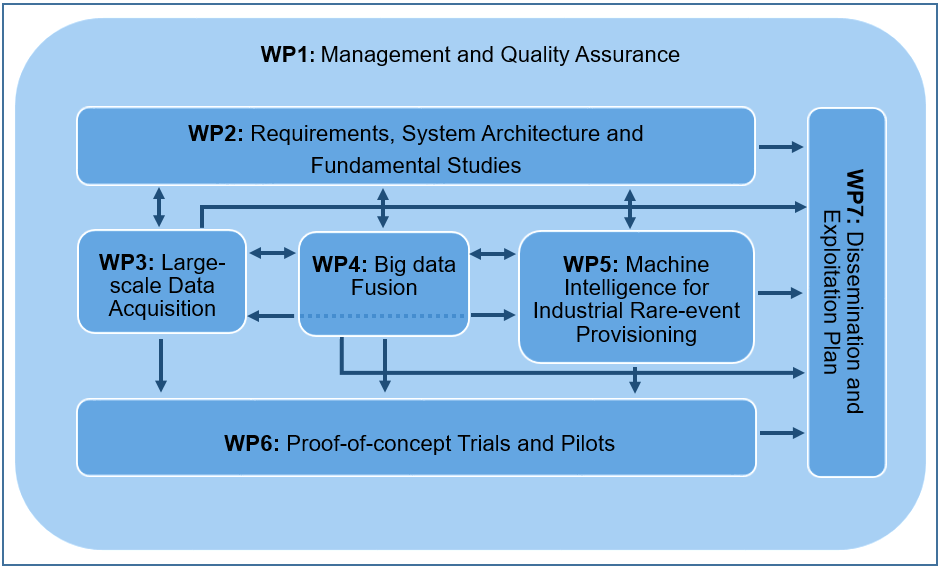
\includegraphics[width=0.8\textwidth]{Images/FIREMAN_pert_diagram.png}
    \caption{FIREMAN WP Diagram}
    \label{fig:wp-diagram}
\end{figure}

WP3, WP4, and WP5 will accomplish the following:
\begin{displayquote}
\enquote{WP3 will focus on the collection and acquisition of heterogeneous data captured by many sensors embedded into various devices and machines in the physical world. This WP will further investigate secure ultra-reliable data transfer and communication while network architecture aspects will be also considered. Aggregated sensor data combined with data fusion, mining, and interpretation will enable efficient control and awareness of the physical processes. This is the objective of WP4 where advanced machine learning techniques will be developed to convert the pre-processed raw sensor data to useful information and allow for preliminary analysis and short-term operational decisions. WP5 will focus on employing big data analytics and artificial intelligence for statistical analysis and knowledge processing to detect/predict/prevent rare events and propose techniques for actuator response.}\citel{fireman-homepage}
\end{displayquote}

This work will focus on WP6 with the goal of demonstrating with real and virtual demonstrations a cohesive system incorporating all the advances made in WP3-WP5.  

\subsubsection{Power Electronics Converter Collaboration}

A collaboration between Aalborg University and LUT University developed as part of the FIREMAN project. The collaboration is designed to explore the implementation and usability of the theoretical work developed in FIREMAN. A major portion of this thesis work is creating the foundation for the creation of a real-time, production anomaly detection solution. This work will present an anomaly detector and preliminary results on a power electronics dataset. In the future, this work can be expanded to an implementation solution in a real power electronic converter.

\subsection{Motivation}

Researchers, engineers, and industry professionals can utilize this work to improve decision making and accuracy in a wide variety of systems. There is currently a gap in the field between the cutting edge theoretical research and applying it to relevant problems and domains. In order to bridge this gap, the researchers must first understand the relevant research, in this case in outlier detection, and then experiment with implementations to determine where it is best suited for practical applications. This will improve the sharing of knowledge and allow multiple domains to benefit from breakthroughs in specific areas. This yields many benefits including, power savings from improved industrial control of electrical process, improved profit from better control over electrical production output, and improved efficiency and accuracy in decision making processes.

The problem is of high importance because current industrial control processes cannot detect or handle anomalies. A conventional power electronics controller cannot determine or compensate for sensor failure or adversarial data. Additionally, applying machine learning in the domain of power systems and industrial processes is a novel idea and rapidly gaining interest. In this domain, it is critical to provide explainability into the machine learning algorithms to confirm they do not react unexpectedly to certain adversarial inputs. If they act erratically it could lead to large negative safety and financial implications in a way that it would not in other fields.


\subsection{Research Problem}

There are many existing techniques for outlier detection in a variety of disciplines from batch machine learning to conventional statistical approaches. These techniques are generally incompatible and siloed. This research proposes to break that barrier and utilize the best techniques and approaches for the problem.

An emerging area of research is applying machine learning techniques to data streams. Streaming or \enquote{online} machine learning algorithms are unable to look at the data multiple times and must act on and update the model as new datapoints arrive. There is a research gap in implementing and testing these algorithms against existing methods for stream anomaly detection (ex. Half-Space Trees) in popular libraries as many of them are two or three years behind current breakthroughs.

These techniques for anomaly detection and machine learning in general are also new in the field of power electronics. Using a machine learning pipeline to improve over an existing static controlled system presents many opportunities. Many machine learning algorithms rely on a black box that will output answers provided inputs. This presents challenges for system critical applications, like power systems, where it is essential to understand why an algorithm is making a specific decision. The algorithms explainability will be analyzed and methods will be proposed so that it is precisely clear why the algorithm is making certain decisions based on input data. This will also be used to analyze what happens when adversarial data enters the system and analyzed from a cyber-security standpoint to design a controller that can defend against potential threats from adversarial inputs.

The resultant algorithm will provide an explainable model that can be used to control industrial processes. The goal is to detect adversarial or anomalous data, and take preventative measures to mitigate its impact.


\subsection{Research Questions}
With this work the researchers hope to answer the following questions:
\begin{itemize}
    \item Why do machine learning techniques lack general adoption in the power systems domain
    \item How can machine learning techniques be used to enable increased explainability, performance, and security in system critical applications?
    \item What existing machine learning libraries are available for streaming time series analysis and how can their performance be improved?
    \item Why is there a lack of standardization in modern datasets to test and benchmark anomaly detection machine learning algorithms?
    \item How can different anomaly detection techniques (conventional statistics, deep learning, etc.) be combined (ensembled) to increase overall prediction capability and accuracy?
\end{itemize}

